%%%%%%%%%%%%%%%%%%%%%%%%%%%%%%%%%%%%%%%%%%%%%%%%%%%%%%%%%%%%%%%%%%%%%%%%%%%%%%%%%%%%%%%%%%%%%%%%%%%%%%%%%%%%%%%%%%%%%%%%%%%%%%%%%%%%%%%%%%%%%%%%%%%%%%%%%%%%%%%%%%%
% Written By Michael Brodskiy
% Class: Embedded Design: Enabling Robotics
% Professor: S. Shazli
%%%%%%%%%%%%%%%%%%%%%%%%%%%%%%%%%%%%%%%%%%%%%%%%%%%%%%%%%%%%%%%%%%%%%%%%%%%%%%%%%%%%%%%%%%%%%%%%%%%%%%%%%%%%%%%%%%%%%%%%%%%%%%%%%%%%%%%%%%%%%%%%%%%%%%%%%%%%%%%%%%%

\documentclass[12pt]{article} 
\usepackage{alphalph}
\usepackage[utf8]{inputenc}
\usepackage[russian,english]{babel}
\usepackage{titling}
\usepackage{amsmath}
\usepackage{graphicx}
\usepackage{enumitem}
\usepackage{amssymb}
\usepackage[super]{nth}
\usepackage{everysel}
\usepackage{ragged2e}
\usepackage{geometry}
\usepackage{multicol}
\usepackage{fancyhdr}
\usepackage{cancel}
\usepackage{siunitx}
\usepackage{physics}
\usepackage{lastpage}
\usepackage{tikz}
\usepackage{mathdots}
\usepackage{yhmath}
\usepackage{cancel}
\usepackage{color}
\usepackage{array}
\usepackage{multirow}
\usepackage{gensymb}
\usepackage{tabularx}
\usepackage{extarrows}
\usepackage{booktabs}
\usetikzlibrary{fadings}
\usetikzlibrary{patterns}
\usetikzlibrary{shadows.blur}
\usetikzlibrary{shapes}

\geometry{top=1.0in,bottom=1.0in,left=1.0in,right=1.0in}
\newcommand{\subtitle}[1]{%
  \posttitle{%
    \par\end{center}
    \begin{center}\large#1\end{center}
    \vskip0.5em}%

}
\usepackage{hyperref}
\hypersetup{
colorlinks=true,
linkcolor=blue,
filecolor=magenta,      
urlcolor=blue,
citecolor=blue,
}

\pagestyle{fancy}

\lfoot[\vspace{-15pt} \hline]{\vspace{-15pt} \hline}
\rfoot[\vspace{-15pt} \hline]{\vspace{-15pt} \hline}
\cfoot[\thepage]{\thepage}
\chead[\textsc{Embedded Systems}]{\textsc{Embedded Systems}}
\lhead[\textsc{EECE2160, CRN: 32014}]{\textsc{EECE2160, CRN: 32014}}
\rhead[\textsc{Page \thepage \hspace{1pt} of \pageref{LastPage}}]{\textsc{Page \thepage \hspace{1pt} of \pageref{LastPage}}}



\pagestyle{fancy}

\title{Design of an Arithmetic Logic Unit}
\date{\today}
\author{Michael Brodskiy\\ \small Professor: S. Shazli}

\begin{document}

\maketitle

\thispagestyle{fancy}

\newpage

\begin{itemize}

    \section{Introduction}

  \item The purpose of this lab is to design an arithmetic-logic unit (ALU) that operates on 8-bit unsigned integers
    
  \item The ALU will support four different operations: addition, subtraction, multiplication, and division 

  \item The results will be displayed in binary format on the LEDs, and also in decimal format on the 7-Segment displays on the DE1-SoC board

    \section{Lab 3 — Preparation of Logic Decisions}

  \item In order to focus on the Schematic designs during this lab session, you need to prepare your designs on paper before implementing them

  \item This lab reuses some components designed in the previous labs including the 8-bit adder and the 7-Segment display with enable

  \item Using a circuit schematics editor to create all connections from scratch is a pretty time-consuming task, so we will be using some pre- designed versions of them existing in libraries included with the Quartus Prime software

  \item Specifically, we will use the Intel FPGA integer Arithmetic IP cores to perform mathematical operations

  \item These components are available on the IP Catalog library located on right side of the Project page as shown on Figure 1; It can also be accessed from the ``Tools Menu'' if you can’t find it

    \begin{figure}[h!]
      \centering
      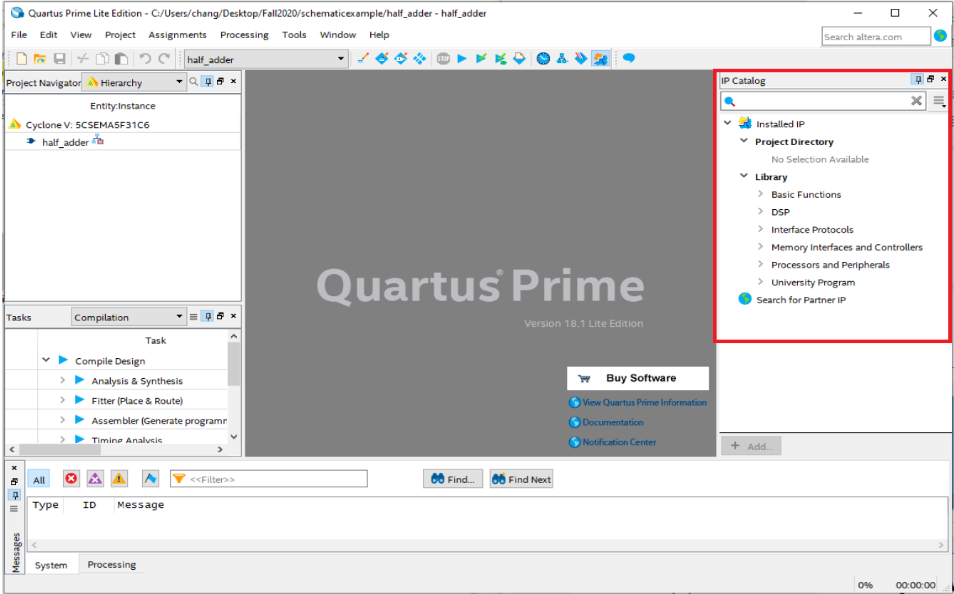
\includegraphics[width=.675\textwidth]{Figures/QPLPP.png}
      \caption{IP Catalog Library}
      \label{fig:1}
    \end{figure}

  \item For this lab, you will need your 7-Segment display with enable files from Lab 2, and the rest of the components will come from the usual components library or the IP Catalog library

    \section{8-Bit Unsigned Integer on the 7-Segment Display}

  \item The ALU design we will build operates on 8-bit unsigned integers (positive integers only) and we would like to see the results in decimal format

  \item That is, the result will be an integer between 0 and 255 for 8-bits. For this part, we will extend our 7-Segment display so that, if given an 8-bit integer, it will display the value (0 to 255) of the integer on up to 3 displays

    \section{Building the ALU Components}

  \item The addition, subtraction, multiplication, and division operations supported by the ALU are implemented in similar LPM modules

  \item You have already created a division block, div8u component created in the previous section

    \section{The 8-Bit ALU Design}

  \item The last step in our hardware design consists in building the complete 8-bit ALU, based on all logic blocks created in this and the previous lab, including the 8-bit adder, 8-bit subtractor, 8-bit multiplier, 8-divider, and 8-bit 4-to-1 MUX

  \item The following logic block shows the interface for the 8-bit ALU:

    \begin{figure}[h!]
      \centering
      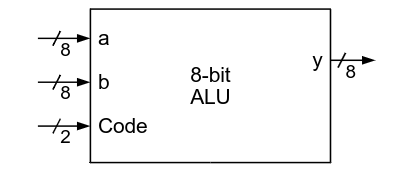
\includegraphics[width=.65\textwidth]{Figures/8BALU.png}
      \caption{8-Bit ALU Design}
      \label{fig:2}
    \end{figure}

  \item As you can see, the 8-bit ALU takes two 8-bit input operands $a$ and $b$, and provides its result in output $y$

  \item A 2-bit input code determines the operation performed by the ALU, hence the value of output $y$, as follows:

    \begin{itemize}

      \item If code is 00, the ALU performs addition. 

      \item If code is 01, the ALU performs subtraction. 

      \item If code is 10, the ALU performs multiplication. 

      \item If code is 11, the ALU performs division 

    \end{itemize}

\end{itemize}

\end{document}

